%%%%%%%%%%%%%%%%%%%%%%%%%%%%%%%%%%%%%%%%%
% Jacobs Landscape Poster
% LaTeX Template
% Version 1.1 (14/06/14)
%
% Created by:
% Computational Physics and Biophysics Group, Jacobs University
% https://teamwork.jacobs-university.de:8443/confluence/display/CoPandBiG/LaTeX+Poster
%
% Further modified by:
% Nathaniel Johnston (nathaniel@njohnston.ca)
%
% This template has been downloaded from:
% http://www.LaTeXTemplates.com
%
% License:
% CC BY-NC-SA 3.0 (http://creativecommons.org/licenses/by-nc-sa/3.0/)
%
%%%%%%%%%%%%%%%%%%%%%%%%%%%%%%%%%%%%%%%%%

%----------------------------------------------------------------------------------------
%	PACKAGES AND OTHER DOCUMENT CONFIGURATIONS
%----------------------------------------------------------------------------------------

\documentclass[final]{beamer}

\usepackage[scale=1.24]{beamerposter} % Use the beamerposter package for laying out the poster
\usepackage[francais]{babel}
\usepackage[utf8]{inputenc}

\usetheme{confposter} % Use the confposter theme supplied with this template

\setbeamercolor{block title}{fg=ngreen,bg=white} % Colors of the block titles
\setbeamercolor{block body}{fg=black,bg=white} % Colors of the body of blocks
\setbeamercolor{block alerted title}{fg=white,bg=dblue!70} % Colors of the highlighted block titles
\setbeamercolor{block alerted body}{fg=black,bg=dblue!10} % Colors of the body of highlighted blocks
% Many more colors are available for use in beamerthemeconfposter.sty

%-----------------------------------------------------------
% Define the column widths and overall poster size
% To set effective sepwid, onecolwid and twocolwid values, first choose how many columns you want and how much separation you want between columns
% In this template, the separation width chosen is 0.024 of the paper width and a 4-column layout
% onecolwid should therefore be (1-(# of columns+1)*sepwid)/# of columns e.g. (1-(4+1)*0.024)/4 = 0.22
% Set twocolwid to be (2*onecolwid)+sepwid = 0.464
% Set threecolwid to be (3*onecolwid)+2*sepwid = 0.708

\newlength{\sepwid}
\newlength{\onecolwid}
\newlength{\twocolwid}
\newlength{\threecolwid}
\setlength{\paperwidth}{48in} % A0 width: 46.8in
\setlength{\paperheight}{36in} % A0 height: 33.1in
\setlength{\sepwid}{0.024\paperwidth} % Separation width (white space) between columns
\setlength{\onecolwid}{0.22\paperwidth} % Width of one column
\setlength{\twocolwid}{0.464\paperwidth} % Width of two columns
\setlength{\threecolwid}{0.708\paperwidth} % Width of three columns
\setlength{\topmargin}{-0.5in} % Reduce the top margin size
%-----------------------------------------------------------

\usepackage{graphicx}  % Required for including images

\usepackage{booktabs} % Top and bottom rules for tables

%----------------------------------------------------------------------------------------
%	TITLE SECTION
%----------------------------------------------------------------------------------------

\title{Calibration en finance : Mélanges de modèles de \bsc{Black-Scholes}} % Poster title

\author{\bsc{Kheldouni} Mohammed-Amine
\\\vspace{1cm} \textbf{ENPC}
\\\vspace{1cm} \textbf{Encadr\'e par :}
Bernard \bsc{Lapeyre}, Professeur à l'Ecole des Ponts ParisTech et Chercheur au CERMICS} % Author(s)

\institute{\vspace{-2cm}}

%----------------------------------------------------------------------------------------

\begin{document}

\addtobeamertemplate{block end}{}{\vspace*{2ex}} % White space under blocks
\addtobeamertemplate{block alerted end}{}{\vspace*{2ex}} % White space under highlighted (alert) blocks

\setlength{\belowcaptionskip}{2ex} % White space under figures
\setlength\belowdisplayshortskip{2ex} % White space under equations

\begin{frame}[t] % The whole poster is enclosed in one beamer frame

\begin{columns}[t] % The whole poster consists of three major columns, the second of which is split into two columns twice - the [t] option aligns each column's content to the top

\begin{column}{\sepwid}\end{column} % Empty spacer column

\begin{column}{\onecolwid} % The first column

%----------------------------------------------------------------------------------------
%	OBJECTIVES
%----------------------------------------------------------------------------------------

\begin{alertblock}{Objectifs}


\end{alertblock}


%----------------------------------------------------------------------------------------
%	INTRODUCTION
%----------------------------------------------------------------------------------------

\begin{block}{Présentation du problème}
  On veut connaître le prix d'une action sur le marché. Une \textit{action} est un titre de propriété délivré par une société de capitaux. \newline
  \textbf{Paramètres :}
  \begin{itemize}
    \item $T$ : La maturité désigne le temps qui sépare la date à laquelle une obligation est émise, et la date à laquelle la valeur nominale de cette obligation est remboursée.
    \item une option :  Produit dérivé qui établit un contrat entre un acheteur et un vendeur.
    \item $S_t$ : Un actif sous-jacent est un actif sur lequel porte une option ou plus largement un produit dérivé.
    \item $r$ : Le taux d'intérêt fixe la rémunération du capital prêté versé par l'emprunteur au prêteur.
    \item $\sigma$ : La volatilité est l'ampleur des variations du cours d'un actif financier. Elle sert de paramètre de quantification du risque de rendement et de prix d'un actif financier. \newline Lorsque la volatilité est élevée, la possibilité de gain est plus importante, mais le risque de perte l'est aussi.
    \item $K$ : Le strike désigne le prix d'exercice d'une option, qui correspond au prix fixé dans le contrat pour l’acquisition ou la cession du sous-jacent.
    \item Call : Le call ou l'option d'achat est une option d'achat sur un instrument financier.
    \item Put : A l'opposé du Call, le Put est l'option de vente de cet instrument.
  \end{itemize}
  Etant donné les paramètres $\sigma$, $T$, $K$, $S_0$ et $r$ on voudrait calculer le prix d'un call ou d'un put sur le marché, pour un actif financier.
\end{block}

%----------------------------------------------------------------------------------------


%----------------------------------------------------------------------------------------

\end{column} % End of the first column

\begin{column}{\sepwid}\end{column} % Empty spacer column

\begin{column}{\twocolwid} % Begin a column which is two columns wide (column 2)

\begin{block}{Modélisation mathématique du marché et problèmes de calibration}

\begin{columns}[t,totalwidth=\twocolwid] % Split up the two columns wide column

\begin{column}{\onecolwid} % The first column within column 2 (column 2.1)

%----------------------------------------------------------------------------------------
%	MATERIALS

\begin{alertblock}{Modèle de \bsc{Black-Scholes}}
  Dans ce modèle, on considére le prix de l'action comme un processus stochastique en temps continu $S_t$. \newline
  \textbf{Hypothèses :}
  \begin{itemize}
    \item  Marchés efficients :
    \begin{itemize}
      \item Pas de coûts de transaction
      \item Pas de restrictions sur le volume de transactions
      \item Pas d'opportunité d'arbitrage
    \end{itemize}
    \item Les rendements du sous-jacent sont gaussiens, stationnaires et indépendants.
    \item Le placement à la banque est sans risque et le taux d'intérêt r est constant.
  \end{itemize}
  \textbf{Equation différentielle stochastique}
  \[ {\color{red} dS_t = \mu S_t dt + \sigma S_t dW_t} \]
On note \begin{itemize}
      \item $S_0$ - La valeur actuelle de l'action sous-jacente.
      \item $T$ - Le temps qu'il reste à l'option avant son échéance (la maturité).
      \item $K$ - Le prix d'exercice fixé par l'option.
      \item $W_t$ - Mouvement Brownien de variance $t$
\end{itemize}
\end{alertblock}

%----------------------------------------------------------------------------------------

\end{column} % End of column 2.1

\begin{column}{\onecolwid} % The second column within column 2 (column 2.2)

%----------------------------------------------------------------------------------------
%	METHODS
%----------------------------------------------------------------------------------------

Le prix théorique d'un call donnant le droit mais pas l'obligation d'acheter l'actif $S$ à la valeur $K$ à la date $T$, est caractérisé par son \textit{payoff}:
$$ (S_T - K)^{+} = \max (S_T -K,0) $$
La formule de Black-Scholes donne le prix d'un Call :
$$ C(S_0,K,r,t,\sigma) = S_0 \phi(d_1)-K \times e^{-rt} \phi(d_2) $$
Avec : \begin{itemize}
\item $\phi$ la fonction de répartition de la loi normale centrée réduite.
\item $d_1 = \frac{1}{\sigma \sqrt{t}} (ln(\frac{S_0}{K})+(r+\frac{1}{2}\sigma^2)t) $
\item $d_2 = d_1 - \sigma \sqrt{t}$
\end{itemize}
Et pour un put, on a un prix théorique par rapport à un \textit{payoff} de $ (S_T - K)^{+}$
\\ \vspace{0.5cm}
Et on a une formule de Black-Scholes pour le prix d'un put :
$$ P(S_0,K,r,t,\sigma) = -S_0 \phi(-d_1)+K \times e^{-rt} \phi(-d_2) $$
%----------------------------------------------------------------------------------------

\end{column} % End of column 2.2

\end{columns} % End of the split of column 2 - any content after this will now take up 2 columns width

\end{block}


%----------------------------------------------------------------------------------------
\vspace{-2cm}
\begin{alertblock}{Algorithmes}

\setbeamercolor{block title}{fg=ngreen,bg=dblue!10} % Colors of the block titles
\setbeamercolor{block body}{fg=black,bg=dblue!10} % Colors of the body of blocks

\begin{columns}[t,totalwidth=0.45\paperwidth] % Split up the two columns wide column again

\begin{column}{\onecolwid} % The first column within column 2 (column 2.1)

%----------------------------------------------------------------------------------------
%	MATHEMATICAL SECTION
%----------------------------------------------------------------------------------------
\begin{block}{Mélange de modèles BS}
  On fixe un nombre $P$ de modèles de Black-Scholes dont on va effectuer un mélange selon une certaine distribution de probabilités $(p_1,p_2,...,p_p)$.
  \newline
  Ainsi on considère le Call (et on fait de même pour le prix d'un Put), à $K$, $r$ et $t$ fixés, de notre mélange comme suit :
  $$ C_m(\lambda, \sigma, p) = \sum^p_{i=1} p_i C(\lambda_i,K,r,t,\sigma_i) $$
\begin{itemize}
  \item $\lambda$ : la liste de taille $P$ des sous-jacents de chacun des modèles considérés.
  \item $\sigma$ : la liste des volatilités
  \item $p$ : la liste des probabilités de tirer chacun des modèles.
\end{itemize}
\end{block}

%----------------------------------------------------------------------------------------

\end{column} % End of column 2.1

\begin{column}{\onecolwid} % The second column within column 2 (column 2.2)

%----------------------------------------------------------------------------------------
%	RESULTS
%----------------------------------------------------------------------------------------

\begin{block}{OPTIM}
    En considérant un vecteur $ \beta_0 = (\lambda,\sigma,p)$ fixé, on obtient par la formule de Black-Scholes les prix d'un Call et d'un Put d'une option qu'on prend européenne par exemple.
    \newline
    En oubliant la valeur $\beta_0$, on peut la retrouver en effectuant une méthode des moindres carrés sur plusieurs prix d'exercice $(K_1,...,K_M)$, minimisant les résidus des prix. Pour un call :
    $$ \min \sum^M_{j=1} (C_{m,j}(\beta)-\alpha_j)^2 $$
    \vspace{-0.3cm}
    $$ s.c. \sum^p_{i=1}p_i = 1 $$
  $\alpha_j$ étant le prix du Call calculé pour $\Beta_0$ pour un \textit{Strike} $K_j$.
\end{block}

%----------------------------------------------------------------------------------------

\end{column} % End of column 2.2

\end{columns} % End of the split of column 2

\end{alertblock}

\end{column} % End of the second column

\begin{column}{\sepwid}\end{column} % Empty spacer column

\setbeamercolor{block title}{fg=ngreen,bg=white} % Colors of the block titles
\setbeamercolor{block body}{fg=black,bg=white} % Colors of the body of blocks

\begin{column}{\onecolwid} % The third column

%----------------------------------------------------------------------------------------
%	CONCLUSION
%----------------------------------------------------------------------------------------

\begin{block}{Conclusion : application à la pharmaceutique}
  \begin{minipage}{0.49\textwidth}
    On prend $P = 2$
    \begin{itemize}
      \item $\lambda = (100,100)$
      \item $\sigma = (0.2, 0.4)$
      \item $p = (0.5,0.5) $
      \item $r = 0$
      \item $K = (50,...150)$
    \end{itemize}
  \end{minipage}

  \begin{minipage}{1.49\textwidth}
  \begin{figure}[!r]
    \vspace{-11cm}
    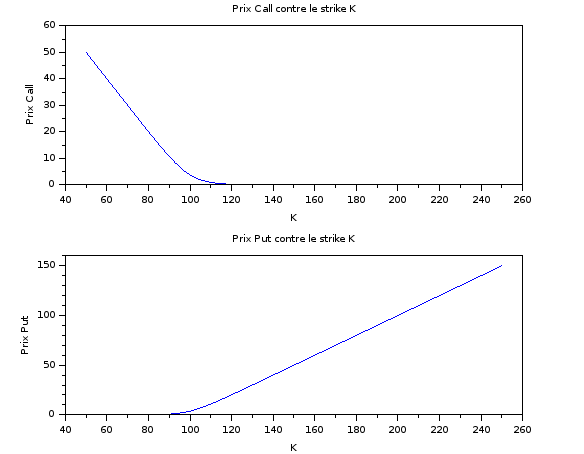
\includegraphics[scale=0.9]{callput.png}
  \end{figure}
  \end{minipage}

  On trouve par la fonction d'optimisation non linéaire de SCILAB, \textit{optim}, un $\beta$ proche de l'optimum :
  $$ \beta_* = (100.001,100.001,0.22,0.38,0.5,0.5) $$
  Toutefois, les erreurs de calibrations étant non négligeables, il a fallu réajuster l'ensemble de recherche des solutions réalisables.
  En effet, même pour $p=2$, il a fallu ajuster un bon intervalle pour le strike $K$, pour que l'optimisation des moindres carrés donne un résultat cohérents avec le $\beta_0$ qu'on a "oublié" pour retrouver par cette méthode.
  \newline
  En augmentant la dimension de l'espace dans lequel vit $\beta$, de dimension $3P$, l'optimisation ne marche plus.
  $$ \Rightarrow \text{C'est un problème de calibration en finance} $$
  Cette fois-ci, connaissant tous les paramètres sauf la volatilité $\sigma$, on va essayer de la retrouver pour un certain sous-jacent du marché. \newline
  Sur le marché, on connait le dernier prix d'un Call/Put émis pour un actif financier et par la formule de Black-Scholes, on inverse l'équation.
  \newline Donc :
  $$ \exists ! \sigma_* s.t. \ \ \ C_{BS}(S_0,K,r,t,\sigma_*) = C_{market} $$
  On appelle cette volatilité, la \textbf{volatilité implicite}.
  Il existe divers méthodes de résolution de l'inversion de la formule de Black-Scholes :
  \begin{itemize}
    \item Méthode de Newton-Raphson de convergence quadratique
    \item La dichotomie de convergence en $\mathcal{O}(log(M))$
  \end{itemize}
  En utilisant la fonction \textit{fsolve} de SCILAB, on obtient un graphe 3D appelé \textbf{la surface de la volatilité} pour les valeurs précédentes avec $M=200$ le nombre de prix d'exercices pris en compte.
    \begin{figure}
      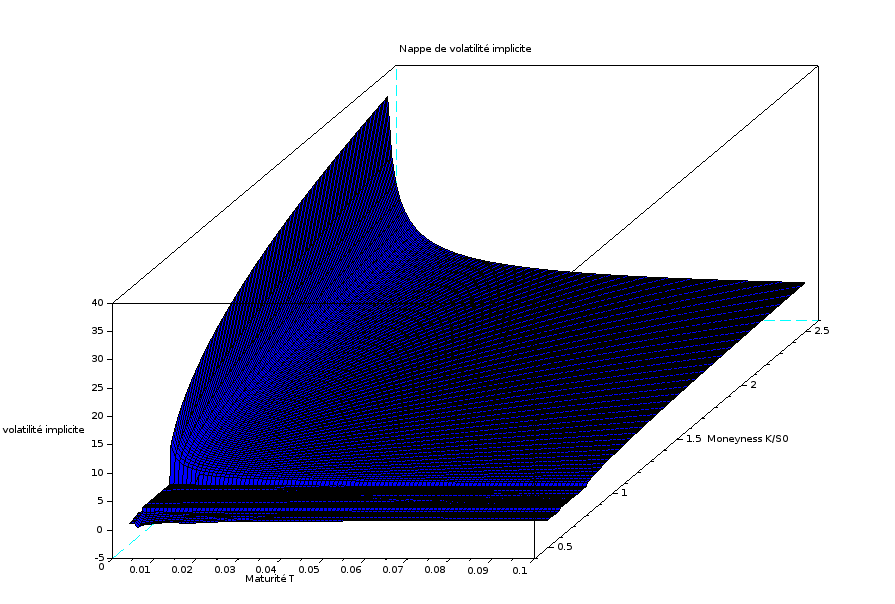
\includegraphics[scale=0.20]{volimpl1.png}
    \end{figure}

\begin{figure}
  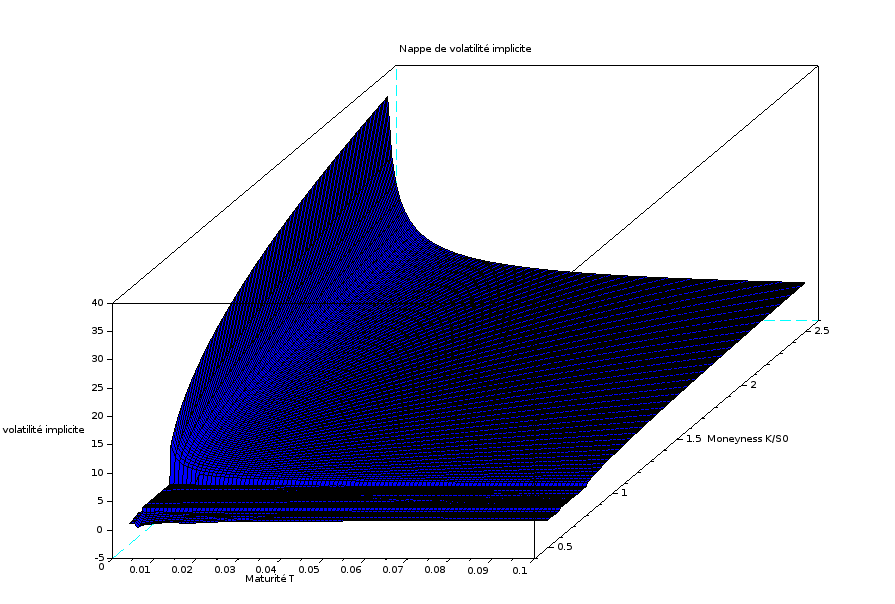
\includegraphics[scale=0.20]{volimpl1.png}
\end{figure}

  On prend $M = 200$ et :

    \[
      \begin{array}{|c|c|}
        \hline
        S_0 & 505.15 \\ \hline
        \sigma_0 & 20\% \\ \hline
        r & 3.3 \% \\ \hline
        K & (500,...,700) \\ \hline
        T & 2 \\ \hline
      \end{array}
    \]
    \begin{figure}
      \vspace{-0.8cm}
      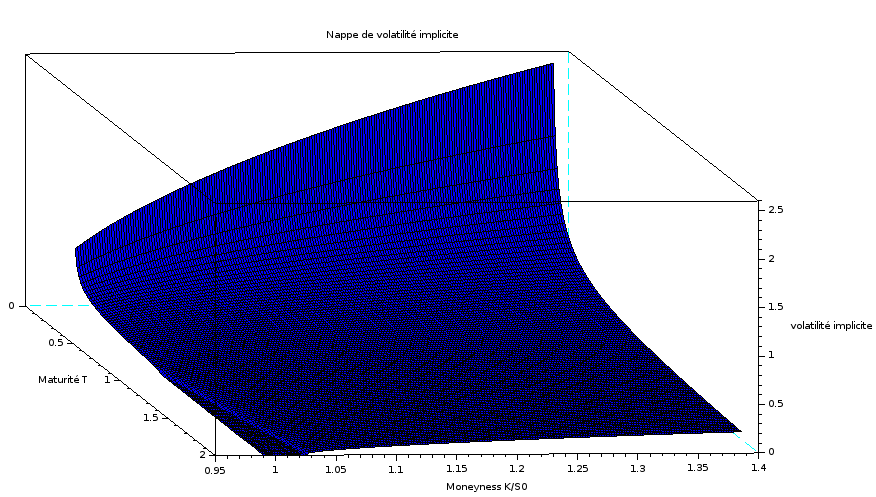
\includegraphics[scale=0.35]{volimpl2.png}
    \end{figure}
\end{block}

%----------------------------------------------------------------------------------------
%	ADDITIONAL INFORMATION
%----------------------------------------------------------------------------------------

%----------------------------------------------------------------------------------------
%	REFERENCES
%----------------------------------------------------------------------------------------

\begin{block}{Références}

\nocite{*} % Insert publications even if they are not cited in the poster
\small{\bibliographystyle{unsrt}
\bibliography{sample}\vspace{0.75in}}
\vspace{-2.5cm}
\end{block}
\begin{center}
  
\includegraphics[scale=0.33]{logos.png}
\end{center}


%\begin{frame}{Bibliographie}
%\begin{itemize}

%   \item \url{https://fr.wikipedia.org/wiki/Maturit%C3%A9_(finance)}
%   \item \url{https://fr.wikipedia.org/wiki/Action_(finance)}
%   \item \url{https://fr.wikipedia.org/wiki/Actif_sous-jacent}
%   \item \url{https://fr.wikipedia.org/wiki/Taux_d%27int%C3%A9r%C3%AAt}
%   \item \url{https://fr.wikipedia.org/wiki/Volatilit%C3%A9_(finance)}
%\end{itemize}
%\end{frame}

%----------------------------------------------------------------------------------------

\end{column} % End of the third column

\end{columns} % End of all the columns in the poster

\end{frame} % End of the enclosing frame

\end{document}
